%\input{frames/dummy}
%\begin{comment}	
\renewcommand{\FileName}{mossoft}

\subsection{Web applet}
\begin{frame}
  \frametitle{Software for Mosaic Displays: Web applet}
  \begin{block}{\large\bfseries Demonstration web applet}
	Go to: \url{http://datavis.ca/online/mosaics/}
	\begin{itemize}
		\item Runs the \emph{current} version of \texttt{mosaics.sas} via a cgi script (perl)
		\item Can:
		\begin{itemize*}
		  \item run \emph{sample} data, 
		  \item \emph{upload} a data file, 
		  \item \emph{enter} data in a form.
		\end{itemize*}
		\item Choose model \emph{fitting} and \emph{display} options (not all supported).
		\item Provides (limited) interaction with the mosaics via javascript
	\end{itemize}
  \end{block}
\end{frame}


\begin{frame}[plain]
\begin{center}
  \includegraphics[width=.9\dispwidth,clip]{fig/mosaic-cgi1a}
%  \includegraphics[width=.95\linewidth]{\vcdguide{mosaic-cgi}}
\end{center}
\end{frame}

\begin{frame}[plain]
\begin{center}
  \includegraphics[width=.9\dispwidth,clip]{fig/mosaic-cgi2a}
\end{center}
\end{frame}
%\end{comment}

\subsection{SAS}
\begin{frame}
  \frametitle{Software for Mosaic Displays: SAS}
  \begin{block}{\large\bfseries SAS software \& documentation}
	\url{http://datavis.ca/mosaics/mosaics.pdf} - User Guide
	\url{http://datavis.ca/books/vcd/macros.html} - Software

   \begin{itemize}
	\item {\large\bfseries Examples}: Many in \VCD{} and on web site

	\item{\large\bfseries \IML{} modules}: \texttt{mosaics.sas}--- Most flexible
      \begin{itemize*}
	  \item Enter frequency table directly in \IML{}, or read from a SAS \Dset{}.
%	  \item Most flexible:
%    	\begin{itemize*}
		\item Select, collapse, reorder, re-label table levels using \IML{} statements
		\item Specify structural 0s, fit specialized models (e.g., quasi-independence)
		\item Interface to models fit using \PROC{GENMOD}
%		\end{itemize*}
      \end{itemize*}
    \end{itemize}
  \end{block}

\end{frame}

\begin{frame}
  \frametitle{Software for Mosaic Displays: SAS}

  \begin{itemize}
	\item{\large\bfseries Macro interface}: \macro{mosaic}, \macro{table}, \macro{mosmat}
	\item{\large\bfseries \macro{mosaic}}--- Easiest to use
%      \begin{itemize*}
%	  \item Easiest to use:
    	\begin{itemize*}
		\item Direct input from a SAS \Dset{}
		\item No knowledge of \IML{} required
		\item Reorder table variables; collapse, reorder table levels with \macro{table}
		\item Convenient interface to \emph{partial mosaics} (\texttt{BY=})
		\end{itemize*}
%	  \end{itemize*}

	\item{\large\bfseries \macro{table}}
      \begin{itemize*}
	  \item Create frequency table from raw data
	  \item Collapse, reorder table categories
	  \item Re-code table categories using SAS formats, e.g., \texttt{1='Male' 2='Female'}
	  \end{itemize*}
	\item{\large\bfseries \macro{mosmat}}
      \begin{itemize*}
	  \item Mosaic matrices--- analog of scatterplot matrix \citep{Friendly:99b}
	  \end{itemize*}
  \end{itemize}
\end{frame}

% slide template
\begin{frame}[fragile]
  \frametitle{\macrot{mosaic} example: Berkeley data}
\begin{Input}[fontsize=\small,label=\fbox{\texttt{berkeley.sas}},baselinestretch=0.7]
title 'Berkeley Admissions data';
proc format;
   value admit 1="Admitted" 0="Rejected"          ;
   value dept  1="A" 2="B" 3="C" 4="D" 5="E" 6="F";
        value $sex  'M'='Male'   'F'='Female';\ignore{$}
data berkeley;
   do dept = 1 to 6;
      do gender = 'M', 'F';
         do admit = 1, 0;
            input freq @@;
            output;
   end; end; end;
\sascomment{/* -- Male --  - Female- */}
\sascomment{/* Admit  Rej  Admit Rej */}
datalines;
     512  313    89   19  \sascomment{/* Dept A */}
     353  207    17    8  \sascomment{/*      B */}
     120  205   202  391  \sascomment{/*      C */}
     138  279   131  244  \sascomment{/*      D */}
      53  138    94  299  \sascomment{/*      E */}
      22  351    24  317  \sascomment{/*      F */}
;
\end{Input}
\end{frame}

\begin{frame}[fragile]
Data set \texttt{berkeley}:
\begin{Output}[gobble=9,baselinestretch=0.7]
                  dept    gender    admit    freq

                    1       M         1       512
                    1       M         0       313
                    1       F         1        89
                    1       F         0        19
                    2       M         1       353
                    2       M         0       207
                    2       F         1        17
                    2       F         0         8
                    3       M         1       120
                    3       M         0       205
                    3       F         1       202
                    3       F         0       391
                    4       M         1       138
                    4       M         0       279
                    4       F         1       131
                    4       F         0       244
                    5       M         1        53
                    5       M         0       138
                    5       F         1        94
                    5       F         0       299
                    6       M         1        22
                    6       M         0       351
                    6       F         1        24
                    6       F         0       317
\end{Output}

\end{frame}

\begin{frame}[fragile]
  \frametitle{\macrot{mosaic} example: Berkeley data}
\begin{Input}[fontsize=\small,label=\fbox{\texttt{mosaic9m.sas}},baselinestretch=0.9]
goptions hsize=7in vsize=7in;
%include catdata(berkeley);
 
\sascomment{*-- apply character formats to numeric table variables;}
%table(data=berkeley, 
    var=Admit Gender Dept,
    weight=freq,
    char=Y, format=admit admit. gender $sex. dept dept.,\ignore{$}
    order=data, out=berkeley);
 
%mosaic(data=berkeley, 
    vorder=Dept Gender Admit, \sascomment{/* reorder variables */}
    plots=2:3,                \sascomment{/* which plots?      */}
    fittype=joint,            \sascomment{/* fit joint indep.  */} 
    split=H V V, htext=3);    \sascomment{/* options           */}
\end{Input}
NB: 
The \texttt{fittype=} argument allows various types of sequential models: joint, conditional, etc.

\end{frame}

\begin{frame}
  \frametitle{\macrot{mosaic} example: Berkeley data}
%% two subfig side-by-side
 \begin{minipage}[t]{.45\textwidth}
  \includegraphics[width=1\linewidth,clip]{fig/mosaic9a2f}
  \\ \centering Two-way, Dept. by Gender
 \end{minipage}%
 \hfill
 \begin{minipage}[t]{.45\textwidth}
  \includegraphics[width=1\linewidth,clip]{fig/mosaic9a3f}
  \\ \centering Three-way, Dept. by Gender by Admit
 \end{minipage}

 
\end{frame}

%\begin{fullversion}
\begin{comment}
\begin{frame}[fragile]
  \frametitle{\IML\ example}
\begin{Verbatim}[fontsize=\small,label=\fbox{\texttt{mosaic9.sas}},baselinestretch=0.7]
proc iml;
   \sascomment{*-- Berkeley Admissions data;}
   dim = \{2 2 6\};
   vnames = \{"Admit" "Gender" "Dept"\};       \sascomment{/* var names   */}
   lnames = \{                                \sascomment{/* level names */}
     "Admitted" "Rejected" " "  " "  " "  " ",
     "Male"  "Female" " "  " "  " "  " ",
     "A" "B" "C" "D" "E" "F"\};
          \sascomment{/* Admit Not Admit Not */}
   table = \{ 512  313,   89   19,
             353  207,   17    8,
             120  205,  202  391,
             138  279,  131  244,
              53  138,   94  299,
              22  351,   24  317\};
   reset storage=mosaic.mosaic;
   \sasemph{load module=_all_;}          \sascomment{*-- Load mosaic modules;}

   title = 'Model: &MODEL';
   plots=2:3;
   fittype='joint';
   \sasemph{run mosaic(dim, table, vnames, lnames, plots, title);}
 quit;
\end{Verbatim}
\end{frame}
\end{comment}
%\end{fullversion}

\begin{frame}[fragile]
  \frametitle{\macrot{mosmat}: Mosaic matrices}
  \vspace{1.5ex}

\begin{Input}[label=\fbox{\texttt{mosmat9m.sas}}]
%include catdata(berkeley);
%mosmat(data=berkeley, 
   vorder=Admit Gender Dept, sort=no);
\end{Input}
	  \vspace{.5ex}
	  \begin{center}
	  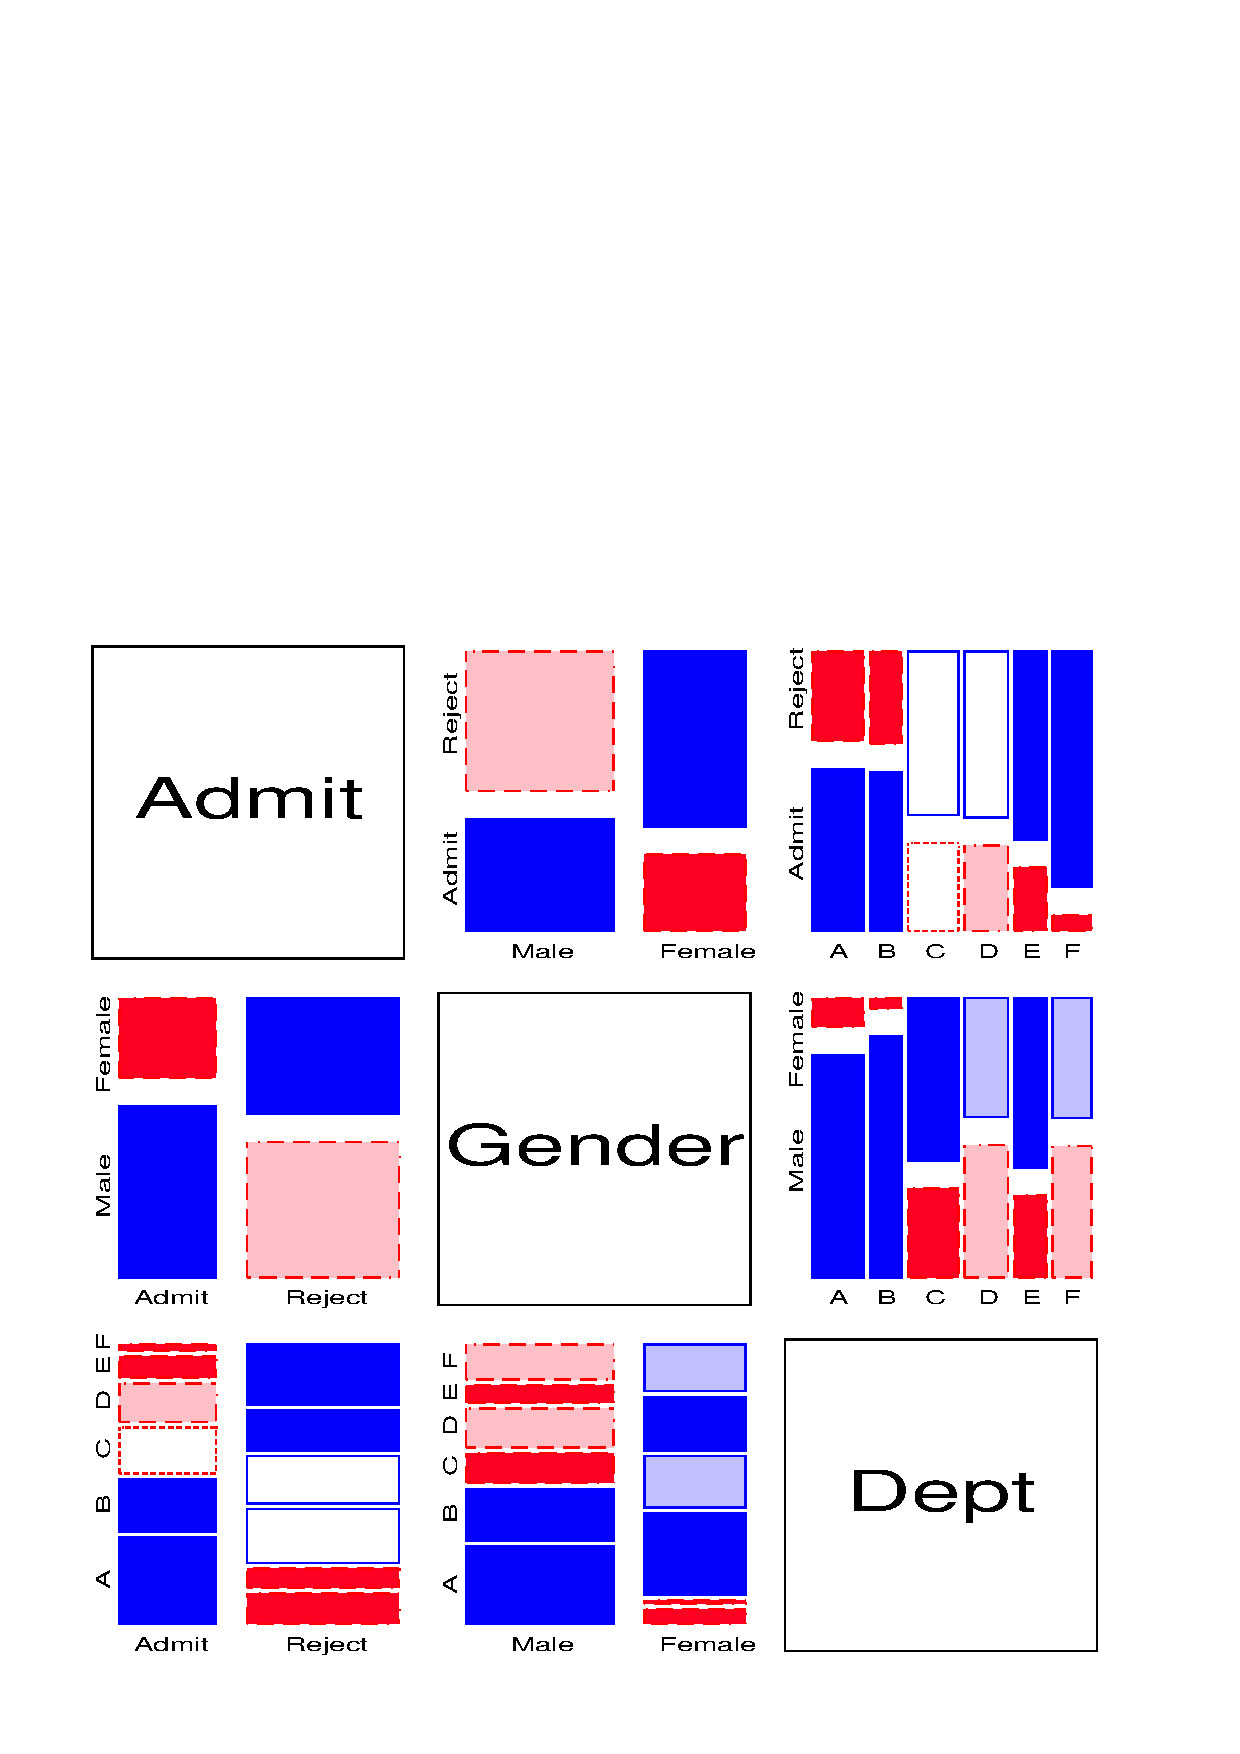
\includegraphics[width=.48\textwidth,clip]{fig/mosmat9a}
	  \end{center}
\end{frame}

\begin{frame}[fragile]
  \frametitle{Partial mosaics}
	  \vspace{1ex}

\begin{Input}[label=\fbox{\texttt{mospart3.sas}},baselinestretch=0.8,fontsize=\footnotesize]
%include catdata(hairdat3s);
%gdispla(OFF);
%mosaic(data=haireye, 
    vorder=Hair Eye Sex, \sasemph{by=Sex}, 
    htext=2, cellfill=dev);
%gdispla(ON);
%panels(rows=1, cols=2);     \sascomment{/* make 2 figs -> 1 */}
\end{Input}

\begin{center}
  \includegraphics[width=.85\dispwidth,clip]{fig/mospart3}
\end{center}
\end{frame}

